\documentclass[11pt]{scrartcl}
\usepackage[utf8]{inputenc}
\usepackage[sexy]{evanchen} 
\usepackage{graphicx}
\graphicspath{{8 Outsource K Math/Gambar/}}


\title{Induksi}
\author{Azzam and Akeyla}
\date{June 2021}

\begin{document}

\maketitle

\renewcommand*\contentsname{Daftar Isi}
\tableofcontents

\newpage

\section{Teorema}
\begin{theorem}
    [Prinsip Induksi]
    Misalkan $P(n)$ adalah sebuah pernyataan yang melibatkan variabel $n$. Jika
    \begin{enumerate}
        \item (Kasus dasar) $P(k_0)$ benar
        \item (Kasus induktif) Jika $P(k)$ benar untuk suatu bilangan bulat $k \geq k_0$, maka $P(k+1)$ juga benar 
    \end{enumerate}
    maka $P(k)$ benar untuk setiap bilangan bulat $k \geq k_0$. 
\end{theorem}

Mari kita coba melihat salah satu persamaan yang umum ditemui:
\begin{example}
    Buktikan bahwa \[1^3 + 2^3 + 3^3 + ... + n^3 = \Big(\frac{n(n+1)}{2}\Big)^2\] untuk setiap bilangan asli $n$.
\end{example}

\begin{proof}[Solusi]

\textbf{(Kasus dasar)} Saat $n = 1$, persamaan $1^3 = \Big(\frac{1(1+1)}{2}\Big)^2$ benar.

\textbf{(Kasus induktif)} Asumsikan persamaan ini berlaku saat $n = k$ untuk $k$ suatu bilangan asli. Artinya, \[1^3 + 2^3 + 3^3 + ... + k^3 = \Big(\frac{k(k+1)}{2}\Big)^2\] Ingin ditunjukkan bahwa persamaan tersebut juga berlaku untuk $n = k + 1$, yakni \[1^3 + 2^3 + 3^3 + ... + (k+1)^3 = \Big(\frac{(k+1)(k+2)}{2}\Big)^2\]
Tentunya, hal ini berlaku, karena

\begin{align*}
    1^3 + 2^3 + 3^3 + ... + k^3 + (k+1)^3 &= \Big(\frac{k(k+1)}{2}\Big)^2 + (k+1)^3 \\
    &= \Big(\frac{(k+1)(k+2)}{2}\Big)^2
\end{align*}

Berdasarkan prinsip induksi, dapat disimpulkan bahwa persamaan yang diberikan di soal memang benar berlaku untuk setiap bilangan asli $n$.

\end{proof}

Tidak hanya dapat digunakan di persamaan, prinsip induksi juga dapat digunakan dalam pernyataan matematis lain.

\begin{example}
    Buktikan bahwa sebuah papan berukuran $2^n \times 2^n$ yang salah satu ubinnya tidak ada dapat ditutupi secara sempurna dengan beberapa tromino-L di bawah ini untuk sembarang $n$ bilangan asli.
    \begin{center}
        \includegraphics[width=0.25\textwidth]{Trominol.png}
    \end{center}
\end{example}

\begin{proof}[Solusi]

\textbf{(Kasus dasar)} Jelas bahwa saat $n = 1$, papan $2^n \times 2^n$ yang salah satu ubinnya tidak ada akan berbentuk tromino-L dan papan ini dapat ditutupi dengan tromino-L. \\
\textbf{(Kasus induktif)} Asumsikan pernyataan soal benar untuk $n = k$ dan akan ditunjukkan kalau pernyataan soal juga benar untuk $n = k + 1$. \\
Perhatikan bahwa papan $2^{k + 1} \times 2^{k + 1}$ dapat dibagi menjadi empat papan $2^k \times 2^k$ seperti pada gambar di bawah ini.

\begin{center}
    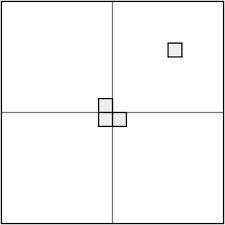
\includegraphics[width=0.25\textwidth]{tiling.png}
\end{center}

Karena ada satu ubin yang tidak ada di papan $2^{k + 1} \times 2^{k+1}$ itu, ubin tersebut pasti terletak di salah satu dari empat bagian papan yang ada. Papan $2^n \times 2^n$ ini akan dapat ditutupi dengan tromino-L berdasarkan asumsi. 

Sementara itu, untuk tiga papan yang lain, taruhlah tromino-L di posisi tengah papan yang besar seperti pada gambar. Tiga papan yang kecil sudah kehilangan satu ubinnya. Berdasarkan asumsi induktif, masing-masing papan ini akan dapat ditutupi dengan tromino-L. Sehingga, dapat disimpulkan bahwa kasus induktif berlaku.

Dari kedua kasus ini, dapat disimpulkan bahwa papan $2^n \times 2^n$ yang kehilangan salah satu ubinnya akan selalu dapat ditutupi dengan tromino-L.

\end{proof}

\section{Variasi}
Prinsip induksi memiliki beberapa variasi yang dapat digunakan untuk menyelesaikan berbagai persoalan.

\begin{theorem}
    [Prinsip Induksi Berlangkah]
    Misalkan $P(n)$ adalah sebuah pernyataan yang melibatkan variabel $n$. Jika
    \begin{enumerate}
        \item (Kasus dasar) $P(k_0), P(k_0 + 1), ..., P(k_0 + m - 1)$ benar
        \item (Kasus induktif) Jika $P(k)$ benar untuk suatu bilangan bulat $k \geq k_0$, maka $P(k+m)$ juga benar 
    \end{enumerate}
    maka $P(k)$ benar untuk setiap bilangan bulat $k \geq k_0$.\\
    Prinsip induksi ini disebut memiliki langkah $m$.
\end{theorem}

Induksi berlangkah ini akan berguna dalam persoalan yang melibatkan barisan rekursif dengan dua suku atau lebih.

\begin{example}
    Sebuah restoran menjual paket berisi $5$ chicken wing dan paket berisi $8$ chicken wing. Buktikan bahwa kita dapat membeli tepat $n$ chicken wing untuk setiap bilangan asli $n > 27$.
\end{example}

\begin{proof}[Solusi]
Gunakan prinsip induksi berlangkah dengan langkah $5$.\\
\textbf{(Kasus dasar)} Kasus dasarnya adalah saat $n = 28, 29, 30, 31$ dan $n = 32$. Perhatikan bahwa $28 = 5 + 5 + 5 + 5 + 8$, $29 = 8 + 8 + 8 + 5$, $30 = 5 + 5 + 5 + 5 + 5 + 5$, $31 = 8 + 8 + 5 + 5 + 5$, dan $32 = 8 + 8 + 8 + 8$.\\
\textbf{(Kasus induktif)} Asumsikan persamaan benar untuk kasus $n = k$, akan dibuktikan bahwa pernyataan tersebut juga benar untuk $n = k + 5$. Hal ini jelas dikarenakan kita hanya perlu menambah satu paket berisi $5$ chicken wings lagi.
Kesimpulannya, setiap bilangan asli $n > 27$ dapat dengan tepat dibeli, seperti yang diharapkan. Pernyataan yang ingin dibuktikan terbukti dengan menggunakan prinsip induksi berlangkah $5$.
\end{proof}

Terdapat juga variasi induksi yang dikenal dengan nama induksi kuat.

\begin{theorem}
    [Prinsip Induksi Kuat]
    Misalkan $P(n)$ adalah suatu pernyataan yang melibatkan variabel $n$. Jika
    \begin{enumerate}
        \item (Kasus dasar) $P(k_0)$ benar
        \item (Kasus induktif) Jika $P(k_0), P(k_0 + 1), P(k_0 + 2), ..., P(k)$ benar untuk suatu bilangan bulat $k \geq k_0$, maka $P(k + 1)$ juga benar
    \end{enumerate}
    maka $P(k)$ benar untuk setiap bilangan bulat $k \geq k_0$. 
\end{theorem}

\begin{example}
    Buktikan bahwa setiap bilangan asli $n$ pasti dapat dinyatakan sebagai penjumlahan bilangan dua berpangkat ($2^k, k \geq 0$ bilangan cacah) yang berbeda.     
\end{example}

\begin{proof}[Solusi]
Dapat digunakan prinsip induksi kuat.\\
\textbf{(Kasus dasar)} Kasus dasar saat $n = 1$. Jelas bahwa $1 = 2^0$. Pernyataan benar untuk kasus ini.\\
\textbf{(Kasus induktif)} Asumsikan pernyataan benar untuk $n = 1, 2, ...,k$, akan dibuktikan bahwa pernyataan juga benar untuk $n = k + 1$.\\
Pilihlah sebuah bilangan dua berpangkat terbesar yang tidak melebihi $k + 1$, sebut saja $2^l$. Perhatikanlah bahwa $0 \leq n + 1 - 2^l < n + 1$. Jika $n + 1 = 2^l$, jelas bahwa $n + 1$ adalah penjumlahan bilangan dua berpangkat yang berbeda. Sehingga, asumsikan bahwa $n + 1 > 2^l$. Perhatikanlah bahwa $n + 1 - 2^l$ adalah bilangan asli yang lebih kecil dari $n + 1$ dan berdasarkan prinsip induksi kuat, merupakan penjumlahan bilangan-bilangan dua berpangkat yang berbeda. Sehingga, $n + 1 - 2^l = 2^{a_1} + 2^{a_2} + ... + 2^{a_m}$ untuk $a_i, i = 1, 2, ..., m$ adalah bilangan cacah yang berbeda-beda. Jadi, $n + 1 = 2^{a_1} + 2^{a_2} + ... + 2^{a_m} + 2^l$. \\
Hal terakhir yang perlu dilakukan adalah menunjukkan bahwa nilai $l$ tidak boleh sama dengan $a_1, a_2, ..., a_m$. Namun, hal ini cukup jelas dari definisi nilai $l$ itu sendiri. Seandainya $l = a_i$, maka
\begin{align*}
    n + 1 &= 2^{a_1} + 2^{a_2} + ... + 2^{a_m} + 2^l\\
    &= 2^{a_1} + 2^{a_2} + ... + 2^{a_m} + 2^{a_i}\\
    &\geq 2^{a_i} + 2^{a_i}\\
    &= 2^{a_i + 1}
\end{align*}
Hal ini menunjukkan bahwa $2^{a_i + 1}$-lah yang seharusnya merupakan bilangan dua berpangkat terbesar yang nilainya tidak melebihi $n + 1$, kontradiktif dengan dipilihnya $l = a_i$.\\
Jadi, dapat disimpulkan bahwa $l$ tidak sama dengan $a_i$ untuk $i = 1, 2, ..., m$. Akibatnya, $n + 1$ dapat dinyatakan sebagai penjumlahan beberapa bilangan dua berpangkat yang berbeda. Berdasarkan prinsip induksi kuat, hal ini berlaku untuk setiap bilangan asli.
\end{proof}

\section{Latihan}
Pada beberapa soal, akan ada hint yang dapat dibaca dengan men-decrypt string hint yang ada. Gunakanlah ASCII code encoding seperti di https://www.dcode.fr/ascii-code.
\begin{problem}
    [1,5] Buktikan bahwa $1^2 \times 2 + 2^2 \times 3 + ... + n^2 \times (n + 1) = \frac{n(n + 1)(n + 2)(3n + 1)}{12}$ untuk setiap bilangan asli $n$.
\end{problem}
    
\begin{problem}
    [1,5] Buktikan bahwa $\frac{1}{2} + \frac{1}{3} + ... + \frac{1}{2^n} \geq \frac{n}{2}$ untuk setiap bilangan asli $n$.
\end{problem}

\begin{problem}
    [2] Misalkan $F_1 = 1, F_2 = 1,$ dan$F_n = F_{n - 1} + F_{n - 2}$ untuk $n \geq 3$. Buktikan bahwa $F_{3n}$ selalu merupakan bilangan genap untuk sembarang $n$  bilangan asli.
\end{problem}

\begin{problem}
    [2,5] Buktikan bahwa $(2021!)^2 > 2021^{2021}$
\end{problem}

\begin{problem}
    [2,5] Buktikan bahwa untuk setiap bilangan asli $n$, bilangan $3^{3^n} + 1$ merupakan hasil perkalian setidaknya $2n + 1$ bilangan prima yang tidak harus berbeda.
\end{problem}

\begin{problem}
    [4,8] Buktikan bahwa untuk setiap bilangan asli $n$, terdapat sebuah bilangan asli $n$ digit yang habis dibagi oleh $5^n$ dan semua digitnya merupakan bilangan ganjil.\\
    (Hint: 63656B206D6F64756C6F20355E6B)
\end{problem}

\begin{problem}
    [3; Vietnam MO 1985] Carilah semua fungsi $f:\mathbb{N} \rightarrow \mathbb{R}$ yang memenuhi ketiga syarat berikut:
    \begin{itemize}
        \item $f(1) = \frac{5}{2}$
        \item Untuk setiap bilangan bulat $x, y$, $f(x)f(y) = f(x + y) + f(x - y)$
        \item $f(0) \neq 0$
    \end{itemize}
\end{problem}

\begin{problem}
    [3,5; Malaysia MO 2018 - Sedikit dimodifikasi] Notasikan $g_n$ untuk $n$ sebuah bilangan asli sebagai faktor ganjil terbesar dari $n$.
    \begin{enumerate}[(a)]
        \item Buktikanlah bahwa $g_{n + 1} + g_{n + 2} + ... + g_{2n}$ adalah bilangan kuadrat untuk setiap bilangan asli $n$
        \item Hitunglah nilai dari $g_1 + g_2 + ... + g_{2048}$
    \end{enumerate}
\end{problem}

\begin{problem}
    [4; Kanada JMO 2020] $(a_n)$ adalah barisan bilangan real positif yang memenuhi $a_1 = 1$ dan $a_{n + 1}^2 + a_{n + 1} = a_n$ untuk setiap bilangn asli $n$. Buktikanlah bahwa untuk setiap bilangan asli $n$, \[a_n \geq \frac{1}{n}\]
\end{problem}

\begin{problem}
    [2; Identitas Catalan] Buktikan bahwa untuk setiap bilangan asli $n$, berlaku \[1 - \frac{1}{2} + \frac{1}{3} - \frac{1}{4} + ... + \frac{1}{2n - 1} - \frac{1}{2n} = \frac{1}{n + 1} + \frac{1}{n + 2} + ... + \frac{1}{2n}\]
\end{problem}

\begin{problem}
    [3?; Klasik dan Tricky] Buktikan bahwa untuk setiap bilangan asli $n$ berlaku ketaksamaan \[\frac{1}{2} \cdot \frac{3}{4}  \cdot ... \cdot \frac{2n - 1}{2n} < \frac{1}{\sqrt{3n}}\]
    (Hint: 67616E746920336E2064692072756173206B616E616E206D656E6A61646920336E202B2031)
\end{problem}

\begin{problem}
    [3,5; Polandia MO 1986 - Sedikit dimodifikasi] Tentukan semua bilangan asli $n$ yang memiliki properti bahwa $n!$ dapat dinyatakan sebagai penjumlahan $n$ buah faktor positif berbeda dari $n!$.
\end{problem}

\begin{problem}
    [2,5; Well-known] Sebanyak $n$ orang berdiri di lapangan untuk bermain melempar balon air. Setiap orang akan melemparkan satu balon air ke orang yang jaraknya terdekat dari posisinya berdiri. Jika $n$ ganjil, buktikan bahwa akan ada orang yang tidak menjadi sasaran lempar 
\end{problem}

\end{document}
